\documentclass{article}
\usepackage{graphicx,float}
\usepackage{amsmath,latexsym,amsfonts,amssymb,amsthm}

\usepackage[utf8]{inputenc}
\usepackage[english]{babel}
\usepackage[letterpaper,top=2cm,bottom=2cm,left=3cm,right=3cm,marginparwidth=1.75cm]{geometry}
\renewcommand{\baselinestretch}{1.667}


\title{Compute Intelligence PS s7 lab 5}
\author{Joris Plaščinskas}
\date{\today}


\begin{document}

\maketitle
\section*{Introduction \& Data}
In this laboratory work I explored SOM neural network. I chose to train the model with Iris dataset and used the code from lab-2 to pre-process the data and make an 'iris.csv' file. The iris dataset contains 150 data-points. Each data-point has 4 features and is classified into 1 of 3 classes.

\section*{Training Algorithm \& Code}
The SOM neural network training algorithm is iterative. During each iteration a random data-point is selected from the train dataset. Next step is to find the best matching unit (BMU) - this is done by calculating the euclidean distance between each neuron and the data-point and selecting the neuron with smallest distance, then the weights of the BMU and other neighboring neurons are updated. The neighboring neurons are the ones that are close to BMU (close by index in the array). The distance for neurons that are considered neighbors gradually decreases. Finally after 'training' the labels have to be assigned to each neuron, this is done by grouping data-points into closest neurons and assigning the most common label to the neuron. The code used for training can be seen in Figure~\ref{fig:train} below.
\begin{figure}[H]
    \centering
    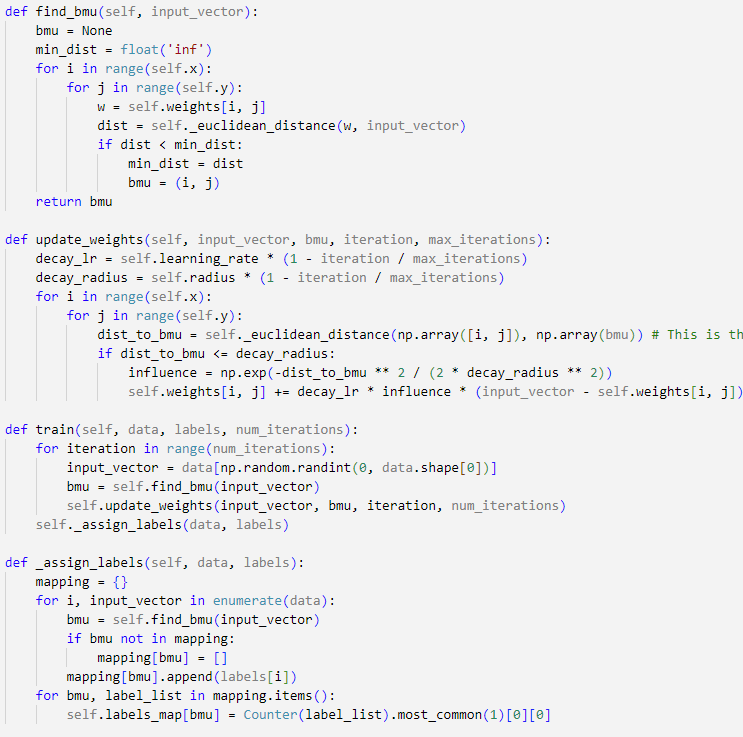
\includegraphics[width=1\textwidth]{SOM-train.png}
    \caption{Training Code}
    \label{fig:train}
\end{figure}

\section*{SOM Visualized}
The Figures \ref{fig:5-labels} \& \ref{fig:10-labels} show which neurons predict which labels in 5x5 \& 10x10 SOM's.
\begin{figure}[H]
    \centering
    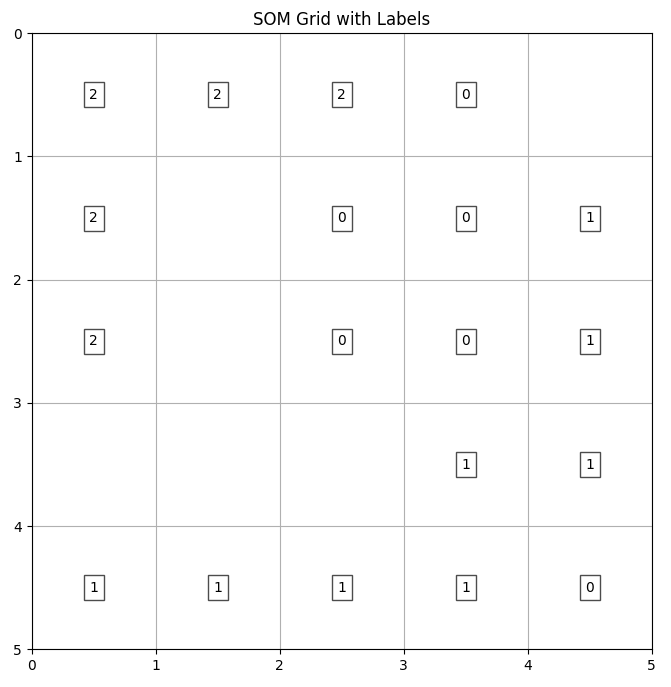
\includegraphics[width=0.8\textwidth]{5-labels.png}
    \caption{5x5 Labels Visualized}
    \label{fig:5-labels}
\end{figure}
\begin{figure}[H]
    \centering
    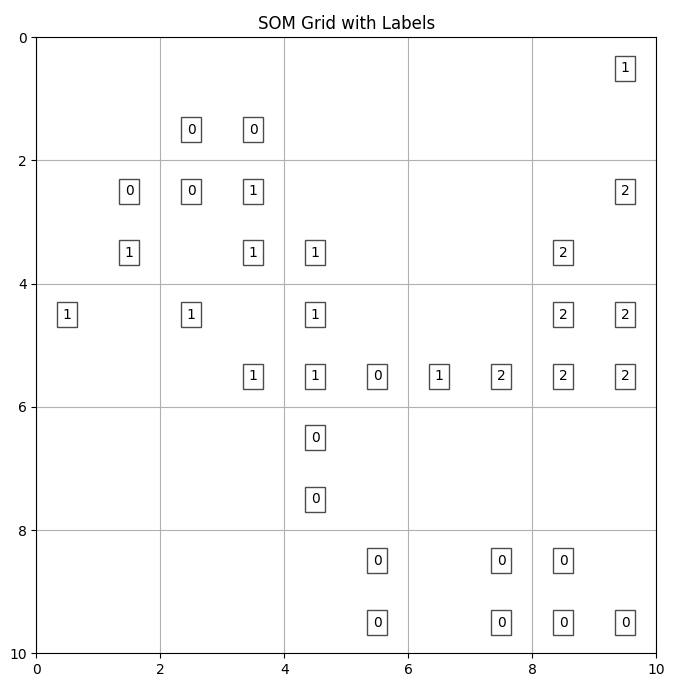
\includegraphics[width=0.8\textwidth]{10-labels.png}
    \caption{10x10 Labels Visualized}
    \label{fig:10-labels}
\end{figure}

\section*{Results}
The 5x5 SOM showed the best results with roughly 95\% accuracy on average. This result basically matches the neural network results from lab-2. The 10x10 SOM also did well with roughly 85\% accuracy. Setting the learning rate high lead to model only classifying one class, while lowering the learning rate slightly improved the performance of 10x10 model. The average distance to BMU for 10x10 map was: 0.085249, and for 5x5: 0.1154321. The new post-lecture maps can be seen below
\begin{figure}[H]
    \centering
    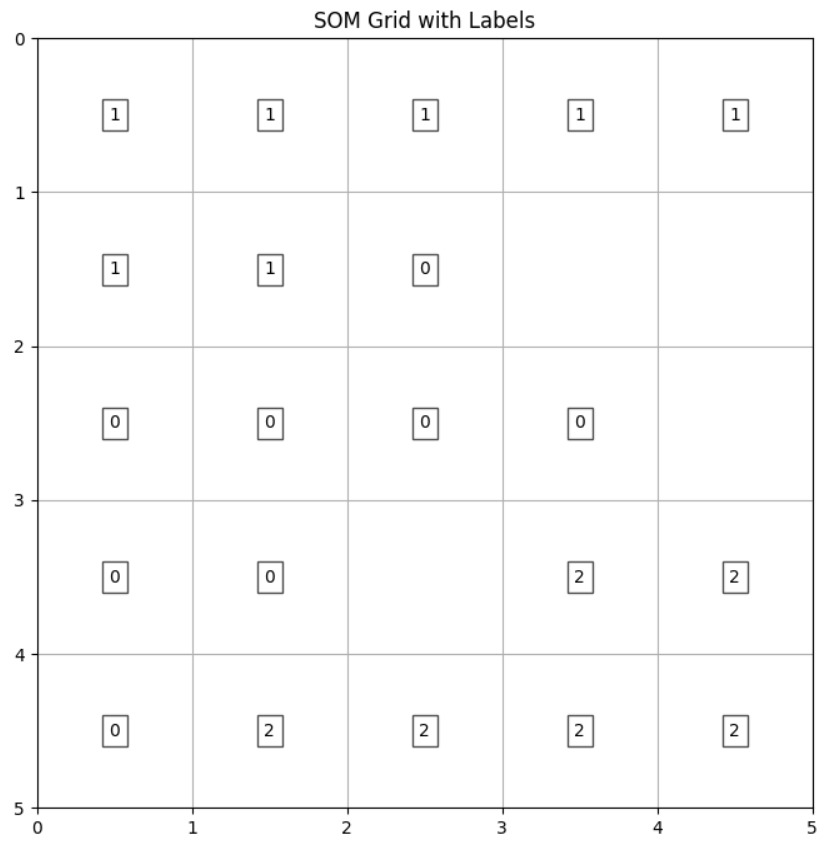
\includegraphics[width=0.8\textwidth]{new-5-5.png}
    \caption{5x5 New Map}
    \label{fig:5-new}
\end{figure}
\begin{figure}[H]
    \centering
    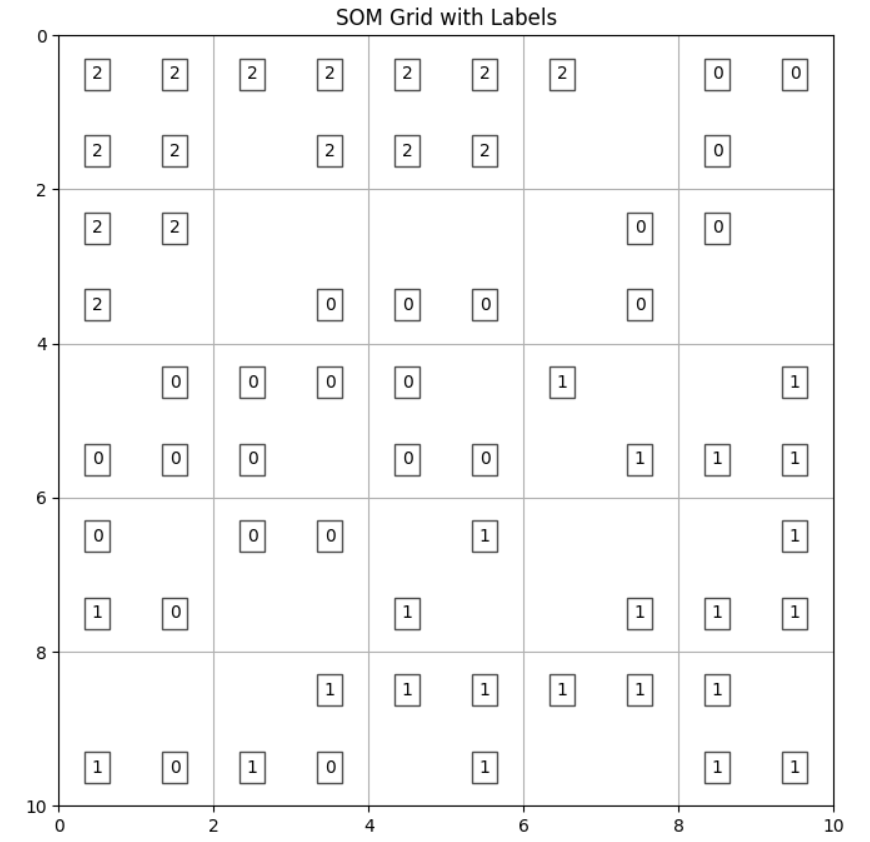
\includegraphics[width=0.8\textwidth]{new-10-10.png}
    \caption{10x10 New Map}
    \label{fig:10-new}
\end{figure}
\end{document}